\PassOptionsToPackage{unicode=true}{hyperref} % options for packages loaded elsewhere
\PassOptionsToPackage{hyphens}{url}
%
\documentclass[
]{article}
\usepackage{lmodern}
\usepackage{amssymb,amsmath}
\usepackage{ifxetex,ifluatex}
\ifnum 0\ifxetex 1\fi\ifluatex 1\fi=0 % if pdftex
  \usepackage[T1]{fontenc}
  \usepackage[utf8]{inputenc}
  \usepackage{textcomp} % provides euro and other symbols
\else % if luatex or xelatex
  \usepackage{unicode-math}
  \defaultfontfeatures{Scale=MatchLowercase}
  \defaultfontfeatures[\rmfamily]{Ligatures=TeX,Scale=1}
\fi
% use upquote if available, for straight quotes in verbatim environments
\IfFileExists{upquote.sty}{\usepackage{upquote}}{}
\IfFileExists{microtype.sty}{% use microtype if available
  \usepackage[]{microtype}
  \UseMicrotypeSet[protrusion]{basicmath} % disable protrusion for tt fonts
}{}
\makeatletter
\@ifundefined{KOMAClassName}{% if non-KOMA class
  \IfFileExists{parskip.sty}{%
    \usepackage{parskip}
  }{% else
    \setlength{\parindent}{0pt}
    \setlength{\parskip}{6pt plus 2pt minus 1pt}}
}{% if KOMA class
  \KOMAoptions{parskip=half}}
\makeatother
\usepackage{xcolor}
\IfFileExists{xurl.sty}{\usepackage{xurl}}{} % add URL line breaks if available
\IfFileExists{bookmark.sty}{\usepackage{bookmark}}{\usepackage{hyperref}}
\hypersetup{
  pdftitle={Oversikt over PROM-skjema for Ukjent sykehus i perioden fra 2017-01-01 til 2017-12-31},
  pdfauthor={Rapporteket},
  pdfborder={0 0 0},
  breaklinks=true}
\urlstyle{same}  % don't use monospace font for urls
\usepackage[margin=1in]{geometry}
\usepackage{graphicx,grffile}
\makeatletter
\def\maxwidth{\ifdim\Gin@nat@width>\linewidth\linewidth\else\Gin@nat@width\fi}
\def\maxheight{\ifdim\Gin@nat@height>\textheight\textheight\else\Gin@nat@height\fi}
\makeatother
% Scale images if necessary, so that they will not overflow the page
% margins by default, and it is still possible to overwrite the defaults
% using explicit options in \includegraphics[width, height, ...]{}
\setkeys{Gin}{width=\maxwidth,height=\maxheight,keepaspectratio}
\setlength{\emergencystretch}{3em}  % prevent overfull lines
\providecommand{\tightlist}{%
  \setlength{\itemsep}{0pt}\setlength{\parskip}{0pt}}
\setcounter{secnumdepth}{-2}
% Redefines (sub)paragraphs to behave more like sections
\ifx\paragraph\undefined\else
  \let\oldparagraph\paragraph
  \renewcommand{\paragraph}[1]{\oldparagraph{#1}\mbox{}}
\fi
\ifx\subparagraph\undefined\else
  \let\oldsubparagraph\subparagraph
  \renewcommand{\subparagraph}[1]{\oldsubparagraph{#1}\mbox{}}
\fi

% set default figure placement to htbp
\makeatletter
\def\fps@figure{htbp}
\makeatother

%\documentclass{article}
\usepackage{xcolor}
\usepackage{sectsty}
\usepackage{marginnote}
\usepackage[norsk]{babel}
\usepackage[left=5cm,%
            right=2cm,%
            top=2.25cm,%
            bottom=2.25cm,%
            headheight=12pt,%
            letterpaper,%
            reversemarginpar,%
            marginparwidth=3.25cm,%
            marginparsep=2em%
            ]{geometry}

% \usepackage[utf8x]{inputenc}
% \usepackage{authblk}
% \usepackage{longtable}
% \usepackage{microtype}
% \usepackage{multicol}
% \usepackage{wasysym}
% \usepackage[raggedright]{titlesec}
% \usepackage[breaklinks]{hyperref}
% \usepackage[color]{changebar}

% Oppsett av fonter
\usepackage[defaultsans]{lato}
\renewcommand{\familydefault}{\sfdefault}

\usepackage[font={rm},labelfont={bf,sf},%
            labelsep=period,%
            skip=4pt,tableposition=top,%
            singlelinecheck=false,justification=centering]{caption}

% Oppsett hode, kne og tå
\usepackage{fancyhdr}  % custom headers/footers
\usepackage{lastpage}  % Number of pages in the document
\pagestyle{fancy}      % Enables the custom headers/footers

% Headers
\makeatletter
\renewcommand{\sectionmark}[1]{\markright{#1}}
\renewcommand{\subsectionmark}[1]{\markright{#1}}
\lhead{\small\sffamily\bfseries\@author}%
\chead{}%
\rhead{\small\sffamily\bfseries\nouppercase{\rightmark}}%
% Footers
\lfoot{\small\sffamily\bfseries\@title}%
\cfoot{}%
\rfoot{\small\sffamily\bfseries\thepage/\pageref{LastPage}}%
\renewcommand{\headrulewidth}{0.1pt}%
\renewcommand{\footrulewidth}{0.1pt}%
\makeatother


% Oppsett tittelside
\makeatletter
\let\authblk@author\author
\let\oldaffil\affil

\usepackage[absolute]{textpos}
\renewcommand{\@maketitle}{%
    \def\@makefnmark{}%
    \begin{textblock*}{\marginparwidth}[1,0]%
      (\dimexpr\Gm@lmargin-\marginparsep,\Gm@tmargin)
      \raggedleft\footnotesize%
      
\includegraphics[width=\hsize]{logo_smerte}%
      \raggedleft\footnotesize%
      {\\ SMERTEREGISTERET er et nasjonalt kvalitetsregister som kvalitesforbedring av smertebehansling som formål. Bla, bla, bla...\par}
      
\includegraphics[width=\hsize]{logo}%
      {\\ RAPPORTEKET er en analysetjenste som tilbyr interaktiv undersøkelse av rådata, rutinemessig utsending av rapporter og visualisering av resultater. Tjenesten utvikles og vedlikeholdes av Nasjonalt servicemiljø for medisinske kvalitetsregistre ved Senter for Klinisk Dokumentasjon og Evaluering (SKDE) og arbeidet finansieres av Helse- og omsorgsdepartementet.}%
    \end{textblock*}
    %
    \begin{textblock*}{\marginparwidth}[1,1]%
      (\dimexpr\Gm@lmargin-\marginparsep,\dimexpr\paperheight-\Gm@bmargin)
      \raggedleft\footnotesize\itshape%
      {\large\rmfamily\upshape\bfseries Om rapporten\par}%
      {\textbf{Bestilt av}\\\@author\par}%
      {\textbf{Produsert av}\\ Rapporteket\par}%
      {\textbf{Dato}\\ dato\par}%
      {\textbf{Tid}\\ tid\par}%
      {\textbf{Fingeravtrykk}\\ fingeravtrykk\par}%
    \end{textblock*}

    {\raggedright\sffamily\bfseries\fontsize{20}{25}\selectfont\@title\par}%
    \vskip10pt
    {\raggedright\@author\par}
    \vskip18pt%
}
\apptocmd{\maketitle}{\thispagestyle{empty}}{}{}
\makeatother
%-----------------------------------------------




% Bruk hf-rager på nivå 1 og 2 overskrifter
\definecolor{hfmork}{RGB}{0,82,155}
\definecolor{hflys}{RGB}{104,174,224}
\subsectionfont{\color{hflys}}
\sectionfont{\color{hfmork}}

\usepackage[explicit]{titlesec}
\titleformat{\section}
  {\color{hfmork}\large\sffamily\bfseries}
  {\thesection}
  {0.5em}
  {#1}
  []
\titleformat{name=\section,numberless}
  {\color{hfmork}\large\sffamily\bfseries}
  {}
  {0em}
  {#1}
  []
\titleformat{\subsection}
  {\color{hflys}\sffamily\bfseries}
  {\thesubsection}
  {0.5em}
  {#1}
  []
\titleformat{\subsubsection}
  {\sffamily\small\bfseries\itshape}
  {\thesubsubsection}
  {0.5em}
  {#1}
  []
\titleformat{\paragraph}[runin]
  {\sffamily\small\bfseries}
  {}
  {0em}
  {#1}

\makeatletter
\titlespacing*{\section}{0pc}{3ex \@plus4pt \@minus3pt}{5pt}
\titlespacing*{\subsection}{0pc}{2.5ex \@plus5pt \@minus2pt}{3pt}
\titlespacing*{\subsubsection}{0pc}{2ex \@plus4.5pt \@minus1.5pt}{2pt}
\titlespacing*{\paragraph}{0pc}{1.5ex \@plus4pt \@minus1pt}{10pt}
\makeatother

% Gjør alle lenker mørkeblå
\definecolor{darkblue}{rgb}{0.0,0.0,0.3}
\hypersetup{colorlinks,breaklinks,linkcolor=darkblue,urlcolor=darkblue,anchorcolor=darkblue,citecolor=darkblue}



% Bruk mørk grå på all annen tekst
\definecolor{text}{RGB}{40,40,40}

\makeatletter
\newcommand{\globalcolor}[1]{%
  \color{#1}\global\let\default@color\current@color
}
\makeatother

\AtBeginDocument{\globalcolor{text}}
\usepackage[english, norsk]{babel}
\usepackage{booktabs}
\usepackage{rotating}
\usepackage{booktabs}
\usepackage{longtable}
\usepackage{array}
\usepackage{multirow}
\usepackage{wrapfig}
\usepackage{float}
\usepackage{colortbl}
\usepackage{pdflscape}
\usepackage{tabu}
\usepackage{threeparttable}
\usepackage{threeparttablex}
\usepackage[normalem]{ulem}
\usepackage{makecell}
\usepackage{xcolor}

\title{Oversikt over PROM-skjema for Ukjent sykehus i perioden fra 2017-01-01
til 2017-12-31}
\author{Rapporteket}
\date{26. november, 2020}

\begin{document}
\maketitle

I denne rapporten finner vi en oversikt over besvarelsene som er gitt
via PROM, både andelen som besvarer og grunnene som er oppgitt til at
besvarelse mangler. I tillegg vises det hvordan svarene fordeler seg på
de ulike spørsmålene for hvert skjema. Det er for tiden fire PROM-skjema
som vises her. Disse er: \emph{pasreg}, \emph{evaluering}, \emph{HADS}
og \emph{opioid}.

Mange av resultatene presenteres i tabeller. Her vises også andelen som
har gitt de ulike svarene. I de tilfellene der andelen ikke summeres til
100 \(\%\) er dette fordi den ``manglende'' prosenten er fjernet fra
oversikten (pga manglende besvarelse og lignende).

En periode kunne man dele ut pasientregistreringsskjema til pasienter
selv om de ikke hadde samtykket fra før. Dersom man valgte å ikke dele
ut pasientregistreringsskjemaene ved manglende samtykke, krysset man av
for «Annet» under «Årsak til manglende utfylling». Derfor vil en del av
annet-kategoriene som vises være store.

\hypertarget{eprom-pasreg}{%
\section{ePROM: pasreg}\label{eprom-pasreg}}

I den valgte tidsperioden fikk tilsammen 1464 pasienter av totalt 2611
tilsendt ePROM-skjema for pasreg. Av de som fikk tilsendt skjema var det
435 pasienter som sendte inn en besvarelse. Dette gir en svarandel på
0.3. Tabell \ref{tab:tabPR} gir en oversikt over registrerte årsaker til
manglende besvarelse for de 1029 som ikke har svart.

\begin{table}

\caption{\label{tab:pasreg}Årsak til manglende utfylling\label{tab:tabPR}}
\centering
\begin{tabular}[t]{l|r|r}
\hline
 & Antall  & Prosent\\
\hline
Tidsmangel behandler & 36 & 2\\
\hline
Tidlig utskrivning & 85 & 6\\
\hline
Kritisk syk/død & 9 & 1\\
\hline
Pasient klarer ikke & 196 & 13\\
\hline
Manglende samtykke & 140 & 10\\
\hline
Ikke besvart ePPROMS & 67 & 5\\
\hline
Annet & 495 & 34\\
\hline
\end{tabular}
\end{table}

\begin{verbatim}
## 
##  Tabellen viser oversikten over søvnproblemer før innleggelse for de 436 pasientene som besvarte spørsmålet:
\end{verbatim}

\begin{verbatim}
## \begin{table}
## 
## \caption{\label{tab:pasreg}}
## \centering
## \begin{tabular}[t]{l|r|r}
## \hline
## Søvnproblemer før innleggelse & Antall  & Prosent\\
## \hline
## Ikke i det hele tatt & 92 & 21\\
## \hline
## I liten grad & 93 & 21\\
## \hline
## I noen grad & 112 & 26\\
## \hline
## I stor grad & 77 & 18\\
## \hline
## I svært stor grad & 60 & 14\\
## \hline
## Vet ikke & 2 & 0\\
## \hline
## \end{tabular}
## \end{table}
\end{verbatim}

\begin{verbatim}
## 
##  Tabellen viser oversikten over søvnproblemer etter innleggelse for de 436 pasientene som besvarte spørsmålet:
\end{verbatim}

\begin{verbatim}
## \begin{table}
## 
## \caption{\label{tab:pasreg}}
## \centering
## \begin{tabular}[t]{l|r|r}
## \hline
## Søvnproblemer etter innleggelse & Antall  & Prosent\\
## \hline
## Ikke i det hele tatt & 20 & 5\\
## \hline
## I liten grad & 69 & 16\\
## \hline
## I noen grad & 136 & 31\\
## \hline
## I stor grad & 125 & 29\\
## \hline
## I svært stor grad & 78 & 18\\
## \hline
## Vet ikke & 8 & 2\\
## \hline
## \end{tabular}
## \end{table}
\end{verbatim}

\begin{verbatim}
## 
##  Figuren viser oversikten over hvor mange ganger pasientene har vært i kontakt med primær- og spesialisthelsetjenesten på grunn av smerter siste år. Det var 326 pasienter som besvarte spørsmålet:
\end{verbatim}

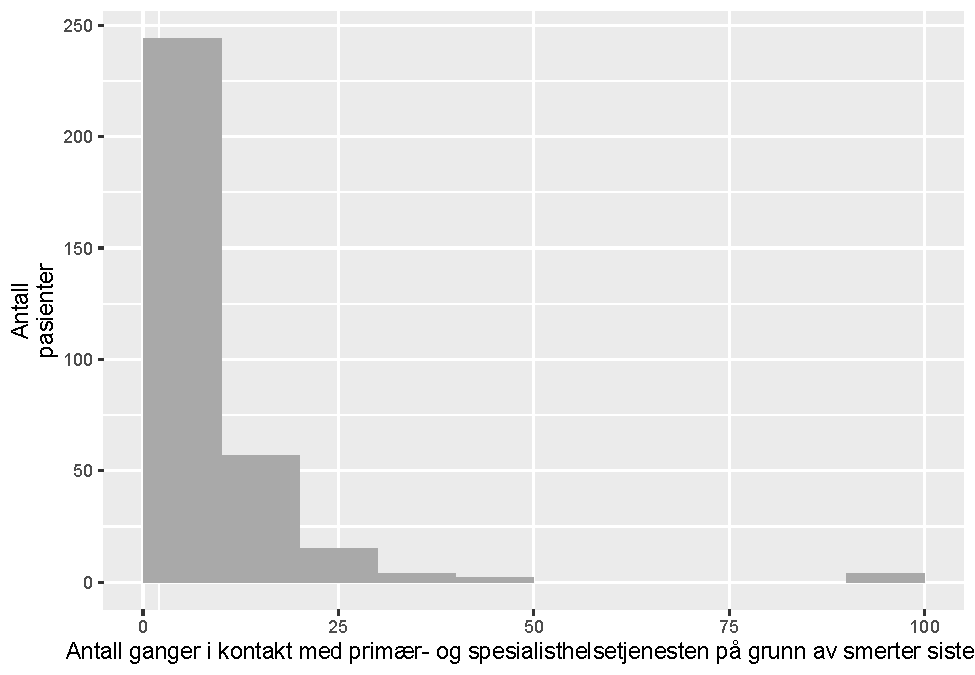
\includegraphics{LokalEprom_files/figure-latex/rest-1.pdf}

\begin{verbatim}
## 
##  Tabellen under viser oversikten over hvor mange av som pasientene tidligere har opplevd belastninger som har krevd behandling av psykolog/psykiater eller liknende. Spørsmålet ble besvart av 436 pasienter.
\end{verbatim}

\begin{verbatim}
## \begin{table}
## 
## \caption{\label{tab:pasreg}}
## \centering
## \begin{tabular}[t]{l|r|r}
## \hline
## Har tidligere opplevd belastninger som har krevd behandling av psykolog/psykiater & Antall  & Prosent\\
## \hline
## Nei & 263 & 60\\
## \hline
## Ja & 165 & 38\\
## \hline
## Vet ikke & 8 & 2\\
## \hline
## \end{tabular}
## \end{table}
\end{verbatim}

\begin{verbatim}
## 
##  Tabellen under viser oversikten over hvor ofte pasientene føler '...det er forferdelig, og jeg at det aldri kommer til å bli bedre'. Spørsmålet ble besvart av 436 pasienter.
\end{verbatim}

\begin{verbatim}
## \begin{table}
## 
## \caption{\label{tab:pasreg}}
## \centering
## \begin{tabular}[t]{l|r|r}
## \hline
## Svar på spørsmålet: ... er det forferdelig, og jeg føler at det aldri kommer til å bli bedre & Antall  & Prosent\\
## \hline
## Aldri & 60 & 14\\
## \hline
## Nesten aldri & 45 & 10\\
## \hline
## Sjelden & 37 & 8\\
## \hline
## Av og til & 133 & 31\\
## \hline
## Ofte & 65 & 15\\
## \hline
## Nesten alltid & 59 & 14\\
## \hline
## Alltid & 29 & 7\\
## \hline
## Vet ikke & 8 & 2\\
## \hline
## \end{tabular}
## \end{table}
\end{verbatim}

\begin{verbatim}
## 
##  Tabellen under viser oversikten over hvor ofte pasientene føler '... det som om jeg ikke holder ut'. Spørsmålet ble besvart av 436 pasienter.
\end{verbatim}

\begin{verbatim}
## \begin{table}
## 
## \caption{\label{tab:pasreg}}
## \centering
## \begin{tabular}[t]{l|r|r}
## \hline
## Svar på spørsmålet: ... føles det som om jeg ikke holder ut & Antall  & Prosent\\
## \hline
## Aldri & 40 & 9\\
## \hline
## Nesten aldri & 43 & 10\\
## \hline
## Sjelden & 40 & 9\\
## \hline
## Av og til & 127 & 29\\
## \hline
## Ofte & 63 & 14\\
## \hline
## Nesten alltid & 76 & 17\\
## \hline
## Alltid & 37 & 8\\
## \hline
## Vet ikke & 10 & 2\\
## \hline
## \end{tabular}
## \end{table}
\end{verbatim}

\hypertarget{eprom-hads}{%
\section{ePROM: HADS}\label{eprom-hads}}

I den valgte tidsperioden fikk tilsammen 1464 pasienter av totalt 2611
tilsendt ePROM-skjema for HADS. Av de som fikk tilsendt skjema var det
435 pasienter som sendte inn en besvarelse. Dette gir en svarandel på
0.3. Under følger en oversikt over registrerte årsaker til manglende
besvarelse for de 1029 som ikke har svart:

\begin{table}

\caption{\label{tab:hads}}
\centering
\begin{tabular}[t]{l|r|r}
\hline
Grunn manglende utfylling HADS & Antall  & Prosent\\
\hline
Tidsmangel behandler & 36 & 2\\
\hline
Tidlig utskrivning & 85 & 6\\
\hline
Kritisk syk/død & 10 & 1\\
\hline
Pasient klarer ikke & 195 & 13\\
\hline
Manglende samtykke & 139 & 9\\
\hline
Ikke besvart ePPROMS & 64 & 4\\
\hline
Annet & 499 & 34\\
\hline
\end{tabular}
\end{table}

Figuren under viser hvordan de 435 aktuelle forløpene fordeles på
depresjonsscore og angstscore i HADS. Poengscorene vurderes som følger:
lavere enn den grønne linjen viser ingen tegn til symptomer, mellom den
grønne og den gule linjen viser milde symptomer, mellom den gule og den
røde linjen er moderate symptomer, mens over den røde er alvorlig
symptomer.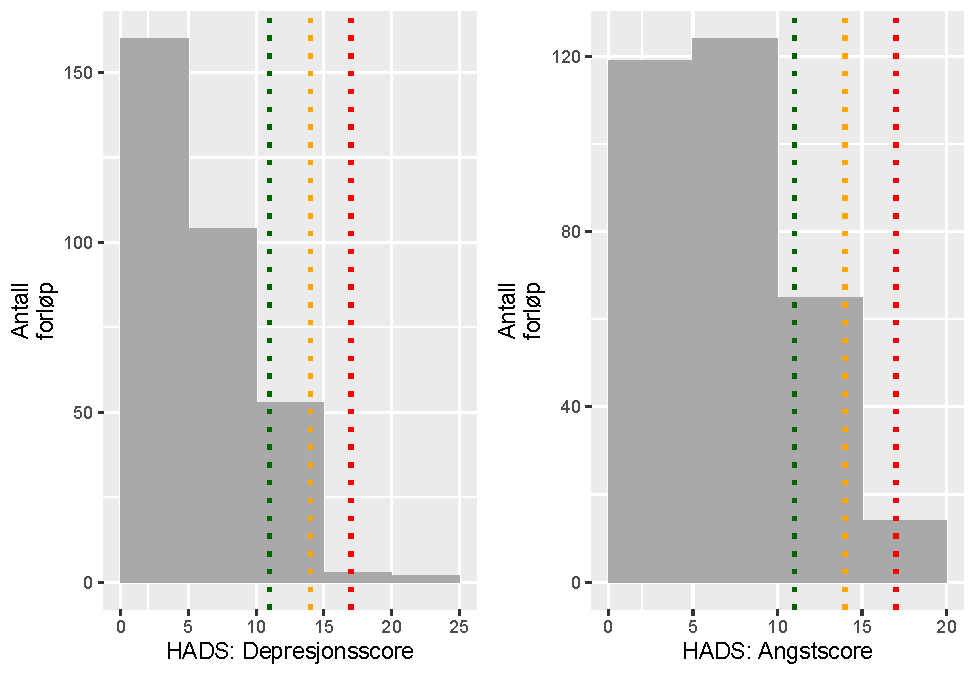
\includegraphics{LokalEprom_files/figure-latex/hads-1.pdf}

\hypertarget{eprom-eval}{%
\subsection{ePROM: Eval}\label{eprom-eval}}

I den valgte tidsperioden fikk tilsammen 1461 pasienter av totalt 2611
tilsendt ePROM-skjema for Eval. Av de som fikk tilsendt skjema var det
380 pasienter som sendte inn en besvarelse. Dette gir en svarandel på
0.26. Under følger en oversikt over registrerte årsaker til manglende
besvarelse for de 1081 som ikke har svart:

\begin{table}

\caption{\label{tab:evalu}}
\centering
\begin{tabular}[t]{l|r|r}
\hline
Grunn manglende utfylling Eval & Antall  & Prosent\\
\hline
Tidsmangel behandler & 39 & 3\\
\hline
Tidlig utskrivning & 93 & 6\\
\hline
Kritisk syk/død & 11 & 1\\
\hline
Pasient klarer ikke & 198 & 14\\
\hline
Manglende samtykke & 139 & 10\\
\hline
Ikke tilstrekkelig antall tilsyn & 19 & 1\\
\hline
Ikke besvart ePPROMS & 65 & 4\\
\hline
Annet & 516 & 35\\
\hline
\end{tabular}
\end{table}

Gjeldende spørsmålet `Husker du at du nylig har vært i kontakt med og
fått behandling av sykehusets smerteteam?' var det 10 pasienter som
svarte ja 0 pasienter som svarte nei og 1451 pasienter som var
registerert med NA/manglende svar.

For det første spørsmålet i Eval: `Siden oppstart av behandling fra
Smerteteamet, er min smertetilstand blitt \ldots{}' finner vi svarene i
tabellen under.

\begin{table}

\caption{\label{tab:evalu}}
\centering
\begin{tabular}[t]{l|r|r}
\hline
Siden oppstart av behandling fra Smerteteamet, er min smertetilstand blitt & Antall  & Prosent\\
\hline
Mye bedre & 168 & 11\\
\hline
Bedre & 114 & 8\\
\hline
Litt bedre & 54 & 4\\
\hline
Uendret & 27 & 2\\
\hline
Litt verre & 7 & 0\\
\hline
Verre & 2 & 0\\
\hline
Mye verre & 4 & 0\\
\hline
Vet ikke & 4 & 0\\
\hline
\end{tabular}
\end{table}

For det andre spørsmålet i Eval: `Siden oppstart av behandling fra
Smerteteamet, er min generelle tilstand blitt \ldots{}' finner vi
svarene i tabellen under.

\begin{table}

\caption{\label{tab:evalu}}
\centering
\begin{tabular}[t]{l|r|r}
\hline
Siden oppstart av behandling fra Smerteteamet, er min generelle tilstand blitt & Antall  & Prosent\\
\hline
Mye bedre & 121 & 8\\
\hline
Bedre & 140 & 10\\
\hline
Litt bedre & 59 & 4\\
\hline
Uendret & 44 & 3\\
\hline
Litt verre & 5 & 0\\
\hline
Verre & 4 & 0\\
\hline
Mye verre & 1 & 0\\
\hline
Vet ikke & 6 & 0\\
\hline
\end{tabular}
\end{table}

For det tredje spørsmålet i Eval: `Hvor fornøyd er du med ivaretakelsen
fra Smerteteamet?' finner vi svarene i tabellen under.

\begin{table}

\caption{\label{tab:evalu}}
\centering
\begin{tabular}[t]{l|r|r}
\hline
Hvor fornøyd er du med ivaretakelsen fra Smerteteamet & Antall  & Prosent\\
\hline
Ikke i det hele tatt & 6 & 0\\
\hline
I liten grad & 12 & 1\\
\hline
I noen grad & 26 & 2\\
\hline
I stor grad & 121 & 8\\
\hline
I svært stor grad & 211 & 14\\
\hline
Vet ikke & 4 & 0\\
\hline
\end{tabular}
\end{table}

For det fjerde spørsmålet i Eval: `Snakket behandlerne i smerteteamet
til deg slik at du forsto dem?' finner vi svarene i tabellen under.

\begin{table}

\caption{\label{tab:evalu}}
\centering
\begin{tabular}[t]{l|r|r}
\hline
Snakket behandlerne i smerteteamet til deg slik at du forsto dem & Antall  & Prosent\\
\hline
I noen grad & 1 & 0\\
\hline
I stor grad & 4 & 0\\
\hline
I svært stor grad & 5 & 0\\
\hline
\end{tabular}
\end{table}

For det femte spørsmålet i Eval: `Har du tillit til smerteteamets
faglige dyktighet?' finner vi svarene i tabellen under.

\begin{table}

\caption{\label{tab:evalu}}
\centering
\begin{tabular}[t]{l|r|r}
\hline
Har du tillit til smerteteamets faglige dyktighet & Antall  & Prosent\\
\hline
I liten grad & 1 & 0\\
\hline
I noen grad & 2 & 0\\
\hline
I stor grad & 3 & 0\\
\hline
I svært stor grad & 4 & 0\\
\hline
\end{tabular}
\end{table}

For det sjette spørsmålet i Eval: `Fikk du tilstrekkelig informasjon og
forklaring om din smertetilstand?' finner vi svarene i tabellen under.

\begin{table}

\caption{\label{tab:evalu}}
\centering
\begin{tabular}[t]{l|r|r}
\hline
Fikk du tilstrekkelig informasjon og forklaring om din smertetilstand & Antall  & Prosent\\
\hline
I noen grad & 3 & 0\\
\hline
I stor grad & 5 & 0\\
\hline
I svært stor grad & 1 & 0\\
\hline
Vet ikke & 1 & 0\\
\hline
\end{tabular}
\end{table}

For det syvende spørsmålet i Eval: `Opplevde du at smertebehandlingen
var tilpasset din situasjon?' finner vi svarene i tabellen under.

\begin{table}

\caption{\label{tab:evalu}}
\centering
\begin{tabular}[t]{l|r|r}
\hline
Opplevde du at smertebehandlingen var tilpasset din situasjon & Antall  & Prosent\\
\hline
I noen grad & 3 & 0\\
\hline
I stor grad & 3 & 0\\
\hline
I svært stor grad & 3 & 0\\
\hline
Vet ikke & 1 & 0\\
\hline
\end{tabular}
\end{table}

For det åttende spørsmålet i Eval: `Var du involvert i avgjørelser som
angikk din smertebehandling?' finner vi svarene i tabellen under.

\begin{table}

\caption{\label{tab:evalu}}
\centering
\begin{tabular}[t]{l|r|r}
\hline
Var du involvert i avgjørelser som angikk din smertebehandling & Antall  & Prosent\\
\hline
Ikke i det hele tatt & 1 & 0\\
\hline
I noen grad & 2 & 0\\
\hline
I stor grad & 5 & 0\\
\hline
I svært stor grad & 2 & 0\\
\hline
\end{tabular}
\end{table}

For det niende spørsmålet i Eval: `Opplevde du at smerteteamets arbeid
var godt organisert?' finner vi svarene i tabellen under.

\begin{table}

\caption{\label{tab:evalu}}
\centering
\begin{tabular}[t]{l|r|r}
\hline
Opplevde du at smerteteamets arbeid var godt organisert & Antall  & Prosent\\
\hline
I liten grad & 1 & 0\\
\hline
I noen grad & 2 & 0\\
\hline
I stor grad & 4 & 0\\
\hline
I svært stor grad & 3 & 0\\
\hline
\end{tabular}
\end{table}

For det tiende spørsmålet i Eval: `Var hjelpen og behandlingen du fikk
av smerteteamet, alt i alt, tilfredsstillende?' finner vi svarene i
tabellen under.

\begin{table}

\caption{\label{tab:evalu}}
\centering
\begin{tabular}[t]{l|r|r}
\hline
Var hjelpen og behandlingen du fikk av smerteteamet, alt i alt, tilfredsstillende & Antall  & Prosent\\
\hline
I noen grad & 4 & 0\\
\hline
I stor grad & 3 & 0\\
\hline
I svært stor grad & 3 & 0\\
\hline
\end{tabular}
\end{table}

For det ellevte spørsmålet i Eval: `Mener du at du på noen måte ble
feilbehandlet av smerteteamet (etter det du selv kan bedømme)?' finner
vi svarene i tabellen under.

\begin{table}

\caption{\label{tab:evalu}}
\centering
\begin{tabular}[t]{l|r|r}
\hline
Mener du at du på noen måte ble feilbehandlet av smerteteamet? & Antall  & Prosent\\
\hline
Ikke i det hele tatt & 6 & 0\\
\hline
I liten grad & 1 & 0\\
\hline
I noen grad & 3 & 0\\
\hline
\end{tabular}
\end{table}

\hypertarget{eprom-opioid}{%
\subsection{ePROM: Opioid}\label{eprom-opioid}}

I den valgte tidsperioden fikk tilsammen 245 pasienter av totalt 2611
tilsendt ePROM-skjema for Opioid. Av de som fikk tilsendt skjema var det
63 pasienter som sendte inn en besvarelse. Dette gir en svarandel på
0.26. Under følger en oversikt over registrerte årsaker til manglende
besvarelse for de 182 som ikke har svart:

\begin{table}

\caption{\label{tab:opi}}
\centering
\begin{tabular}[t]{l|r|r}
\hline
Grunn manglende utfylling Opioid & Antall  & Prosent\\
\hline
Kritisk syk/død & 1 & 0\\
\hline
Pasient klarer ikke & 8 & 3\\
\hline
Manglende samtykke & 107 & 44\\
\hline
Ikke besvart ePPROMS & 48 & 20\\
\hline
Annet & 18 & 7\\
\hline
\end{tabular}
\end{table}

Det er 54 pasienter som svarte ja på at de er utskrevet av sykehus, mens
9 pasienter svarte nei. Samtidig svarer 48 av de som svarte ja at de har
brukt sterke smertestillende medikamenter etter at de ble skrevet ut fra
sykehuset.

I tabellen under vises en oversikt over hvilke medikamenter som har
blitt brukt av pasientene etter utskrivelse.

\begin{table}

\caption{\label{tab:opi}}
\centering
\begin{tabular}[t]{l|r|r}
\hline
  & Antall ja & Antall nei\\
\hline
DolcontinMalfin & 14 & 49\\
\hline
FentanylplDurogesicpl & 7 & 48\\
\hline
Metadon & 1 & 48\\
\hline
Morfin & 15 & 49\\
\hline
Norspanplaster & 4 & 48\\
\hline
OxynormOxykodon & 21 & 49\\
\hline
OxyxontinReltebon & 9 & 48\\
\hline
Palexia & 1 & 48\\
\hline
PalladonHydromorfon & 0 & 48\\
\hline
Paralginforte & 4 & 48\\
\hline
Buprenorfin & 0 & 48\\
\hline
Targiniq & 3 & 48\\
\hline
Tramadolvarianter & 6 & 48\\
\hline
Andre & 4 & 50\\
\hline
Usikker & 3 & 48\\
\hline
\end{tabular}
\end{table}

Videre følger en oversikt over ulike spørsmål tilknyttet bruk og
nedtrapping av medikamentene.

\begin{table}

\caption{\label{tab:opi}}
\centering
\begin{tabular}[t]{l|r|r}
\hline
Bruker du fortsatt noen av disse medikamentene? & Antall  & Prosent\\
\hline
Nei & 11 & 4\\
\hline
Ja, i samme dosering & 17 & 7\\
\hline
Ja, i lavere dosering & 20 & 8\\
\hline
\end{tabular}
\end{table}

\begin{table}

\caption{\label{tab:opi}}
\centering
\begin{tabular}[t]{l|r|r}
\hline
Fikk du informasjon om nedtrapping av sterke smertestillende medikamenter? & Antall  & Prosent\\
\hline
Nei & 11 & 4\\
\hline
Ja & 37 & 15\\
\hline
\end{tabular}
\end{table}

\begin{table}

\caption{\label{tab:opi}}
\centering
\begin{tabular}[t]{l|r|r}
\hline
Av hvem fikk du informasjon om nedtrapping av sterke smertestillende medikamenter? & Antall  & Prosent\\
\hline
Smerteteam & 19 & 8\\
\hline
Annet helsepersonell & 7 & 3\\
\hline
Begge & 10 & 4\\
\hline
Vet ikke & 1 & 0\\
\hline
\end{tabular}
\end{table}

Det er 26 pasienter som fikk muntlig info om nedtrapping, mens 48
pasienter svarte at de ikke fikk det. Samtidig svarer 24 pasienter at de
fikk skriftlig nedtrappingsplan, mens 48 svarer at de ikke fikk det. I
tillegg svarer 8 pasienter at de fikk utdelt infobrosjyre om
nedtrapping, mens 48 svarer at de ikke fikk den utdelt.

\begin{table}

\caption{\label{tab:opi}}
\centering
\begin{tabular}[t]{l|r|r}
\hline
Klarte du å følge anbefalingene for bruk og nedtrapping av medikamentene? & Antall  & Prosent\\
\hline
Ja & 21 & 9\\
\hline
Nei, lenger enn anbefalt & 11 & 4\\
\hline
Nei, har ikke kunnet trappe ned & 2 & 1\\
\hline
Ja, raskere & 3 & 1\\
\hline
\end{tabular}
\end{table}

\begin{table}

\caption{\label{tab:opi}}
\centering
\begin{tabular}[t]{l|r|r}
\hline
Opplevde du plagsomme abstinenssymptomer (svetting/frysing, uro, smerter, diaré, rennende nese) etter at du ble skrevet ut fra sykehuset? & Antall  & Prosent\\
\hline
Nei & 30 & 12\\
\hline
Ja & 9 & 4\\
\hline
Usikker & 9 & 4\\
\hline
\end{tabular}
\end{table}

\begin{table}

\caption{\label{tab:opi}}
\centering
\begin{tabular}[t]{l|r|r}
\hline
Forstod du at det var abstinenssymptomer? & Antall  & Prosent\\
\hline
Ja & 8 & 3\\
\hline
Usikker & 1 & 0\\
\hline
\end{tabular}
\end{table}

\begin{table}

\caption{\label{tab:opi}}
\centering
\begin{tabular}[t]{l|r|r}
\hline
Visste du hva du kunne gjøre med problemet? & Antall  & Prosent\\
\hline
Nei & 2 & 1\\
\hline
Ja & 6 & 2\\
\hline
Usikker & 1 & 0\\
\hline
\end{tabular}
\end{table}

\begin{table}

\caption{\label{tab:opi}}
\centering
\begin{tabular}[t]{l|r|r}
\hline
Opplevde du plagsom tretthet eller følelse av å være medikamentpåvirket etter at du ble skrevet ut fra sykehuset? & Antall  & Prosent\\
\hline
Nei & 36 & 15\\
\hline
Ja & 12 & 5\\
\hline
\end{tabular}
\end{table}

\begin{table}

\caption{\label{tab:opi}}
\centering
\begin{tabular}[t]{l|r|r}
\hline
Visste du hva du kunne gjøre med problemet? & Antall  & Prosent\\
\hline
Nei & 3 & 1\\
\hline
Ja & 3 & 1\\
\hline
Vet ikke & 6 & 2\\
\hline
\end{tabular}
\end{table}

\begin{table}

\caption{\label{tab:opi}}
\centering
\begin{tabular}[t]{l|r|r}
\hline
Fikk du informasjon om sterke smertestillende medikamenter og bilkjøring? & Antall  & Prosent\\
\hline
Nei & 12 & 5\\
\hline
Ja & 32 & 13\\
\hline
Ikke aktuelt & 4 & 2\\
\hline
\end{tabular}
\end{table}

\begin{table}

\caption{\label{tab:opi}}
\centering
\begin{tabular}[t]{l|r|r}
\hline
Av hvem fikk du informasjon om sterke smertestillende medikamenter og bilkjøring? & Antall  & Prosent\\
\hline
Smerteteam & 6 & 2\\
\hline
Annet helsepersonell & 6 & 2\\
\hline
Begge & 19 & 8\\
\hline
Vet ikke & 1 & 0\\
\hline
\end{tabular}
\end{table}

Det er 28 pasienter som fikk muntlig info om medikamenter og bilkjøring,
mens 48 pasienter svarte at de ikke fikk det. Samtidig svarer 6
pasienter at de fikk skriftlig info om medikamenter og bilkjøring, mens
48 svarer at de ikke fikk det. I tillegg svarer 11 pasienter at de fikk
utdelt infobrosjyre «Sterke smertestillende -- informasjon om kortvarig
bruk og nedtrapping», mens 48 svarer at de ikke fikk den utdelt.

\begin{table}

\caption{\label{tab:opi}}
\centering
\begin{tabular}[t]{l|r|r}
\hline
Visste du hvor du kunne henvende deg ved spørsmål om bruk av de smertestillende medikamentene? & Antall  & Prosent\\
\hline
Nei & 12 & 5\\
\hline
Ja & 33 & 13\\
\hline
Usikker & 3 & 1\\
\hline
\end{tabular}
\end{table}

\end{document}
